\section{Experiments and Results}

We conducted 192 experiments across seven experimental phases (B1--B7) to systematically isolate the contribution of pooling strategy, layer fusion, adapter modules, data augmentation, model fine-tuning, and cross-corpus transfer on children's speech emotion recognition. All experiments use WavLM Base as the SSL backbone with a 12-layer fusion module and SEMLP classifier. Unless stated otherwise, the backbone is frozen, training uses 100 epochs with early stopping (patience=15), and results are reported as the mean of three random seeds (42, 123, 456) with standard deviation.

\subsection{Baseline: Pooling Strategy Across Corpora (B1)}

We first establish baselines by evaluating three pooling strategies---mean pooling, self-attention pooling, and prosody-guided pooling---on each of the three corpora. Table~\ref{tab:b1} reports the 3-seed results.

\begin{table}[h]
\centering
\caption{Pooling strategy baselines across corpora (B1, frozen WavLM, 3 seeds).}
\label{tab:b1}
\begin{tabular}{llccc}
\toprule
\textbf{Exp} & \textbf{Corpus} & \textbf{Pooling} & \textbf{WA (mean$\pm$std)} & \textbf{Best Seed} \\
\midrule
E1-02 & C-BESD & Self-Attention & 92.92$\pm$2.15\% & 95.14\% \\
E1-01 & C-BESD & Mean           & 79.56$\pm$1.14\% & 80.55\% \\
E1-03 & C-BESD & Prosody        & 87.38$\pm$0.79\% & 88.15\% \\
\addlinespace
E1-05 & FAU Aibo & Self-Attention & 67.81$\pm$2.15\% & 69.34\% \\
E1-04 & FAU Aibo & Mean           & 64.40$\pm$0.76\% & 65.27\% \\
E1-06 & FAU Aibo & Prosody        & 65.38$\pm$1.23\% & 66.80\% \\
\addlinespace
E1-08 & IEMOCAP & Self-Attention  & 65.16$\pm$1.34\% & 66.38\% \\
E1-07 & IEMOCAP & Mean            & 58.86$\pm$1.66\% & 60.69\% \\
E1-09 & IEMOCAP & Prosody         & 56.22$\pm$0.66\% & 56.60\% \\
\bottomrule
\end{tabular}
\end{table}

Self-attention pooling consistently outperforms alternatives across all corpora, achieving 92.92\% on C-BESD (children's acted speech), 67.81\% on FAU Aibo (children's spontaneous speech), and 65.16\% on IEMOCAP (adult acted speech). The 25-percentage-point gap between C-BESD and FAU Aibo---both children's corpora---cannot be explained by pooling strategy alone. Mean pooling underperforms self-attention substantially on C-BESD ($-$13.4pp) but narrows on FAU and IEMOCAP.

\subsection{Cross-Corpus Zero-Shot Transfer Reveals Distribution Shift (B2)}

To quantify the distribution gap between corpora, we evaluate zero-shot transfer: models trained on one corpus are tested directly on another without fine-tuning. Table~\ref{tab:b2} reports the best transfer direction per source-target pair.

\begin{table}[h]
\centering
\caption{Zero-shot cross-corpus transfer (B2, single run, best pooling per direction).}
\label{tab:b2}
\begin{tabular}{lllc}
\toprule
\textbf{Exp} & \textbf{Source $\rightarrow$ Target} & \textbf{Pooling} & \textbf{WA} \\
\midrule
E3-14 & IEMOCAP $\rightarrow$ C-BESD  & Self-Attention & 34.68\% \\
E3-17 & IEMOCAP $\rightarrow$ FAU     & Self-Attention & 33.71\% \\
E3-10 & FAU $\rightarrow$ IEMOCAP     & Mean           & 35.47\% \\
E3-07 & FAU $\rightarrow$ C-BESD      & Mean           & 23.52\% \\
E3-02 & C-BESD $\rightarrow$ IEMOCAP  & Self-Attention & 33.47\% \\
E3-05 & C-BESD $\rightarrow$ FAU      & Self-Attention & 19.17\% \\
\bottomrule
\end{tabular}
\end{table}

Zero-shot performance collapses across all directions (best: 35.47\%), confirming severe distribution shift between corpora. The C-BESD $\rightarrow$ FAU direction is the most degraded (19.17\%), indicating that acted-to-spontaneous transfer is particularly challenging for children's speech. Critically, neither source nor target domain alone predicts transfer success---the interaction between specific corpora dominates.

\subsection{Data Augmentation Provides Marginal Benefit (B3)}

We tested four augmentation conditions on all three corpora: C1 (baseline, no augmentation), C2 (adult-domain noise injection), C3 (child-domain constrained augmentation), and C4 (mixed-domain augmentation). Table~\ref{tab:b3} summarizes the 3-seed results on FAU Aibo.

\begin{table}[h]
\centering
\caption{Augmentation sensitivity on FAU Aibo (B3, 3 seeds).}
\label{tab:b3}
\begin{tabular}{lcc}
\toprule
\textbf{Condition} & \textbf{WA (mean$\pm$std)} & \textbf{$\Delta$ vs C1} \\
\midrule
C1 (baseline)  & 67.81$\pm$2.15\% & --- \\
C3 (child aug) & 68.38$\pm$1.31\% & +0.57pp \\
C2 (adult aug) & 61.00$\pm$0.79\% & $-$6.81pp \\
C4 (mixed aug) & 58.57$\pm$0.33\% & $-$9.24pp \\
\bottomrule
\end{tabular}
\end{table}

Child-domain augmentation (C3) yields a marginal positive effect (+0.57pp), while adult-domain (C2) and mixed-domain (C4) augmentations cause significant degradation ($-$6.8 to $-$9.2pp). This asymmetric effect suggests that augmentation is only beneficial when the injected distribution matches the target domain.

\subsection{Layer Fusion Has Negligible Impact (B4)}

We conducted a 54-experiment ablation of layer fusion strategies---last layer, weighted fusion, and single-layer selection (L1--L12)---across all three corpora. On C-BESD, all fusion variants converged within a 2pp band (90.7--92.9\%), with single layers L$\geq$7 performing equivalently to weighted fusion. On FAU and IEMOCAP, the same pattern held with even tighter variance. We conclude that layer fusion strategy is not a meaningful design choice: any layer L$\geq$7 suffices.

\subsection{Unfreezing WavLM Provides Consistent Gains (B5)}

We compared frozen versus unfrozen WavLM across all three corpora (Table~\ref{tab:b5}).

\begin{table}[h]
\centering
\caption{Unfreeze comparison (B5, 3 seeds).}
\label{tab:b5}
\begin{tabular}{llcc}
\toprule
\textbf{Exp} & \textbf{Corpus} & \textbf{WA (frozen)} & \textbf{WA (unfrozen)} \\
\midrule
E2-01 & C-BESD   & 92.92\% & \textbf{96.91$\pm$0.53\%} \\
E2-02 & FAU Aibo & 67.81\% & \textbf{76.02$\pm$0.68\%} \\
E2-03 & IEMOCAP  & 65.16\% & \textbf{66.36$\pm$3.30\%} \\
\bottomrule
\end{tabular}
\end{table}

Unfreezing provides the largest absolute gain on FAU Aibo (+8.2pp), moderate gain on C-BESD (+4.0pp, approaching ceiling), and minimal gain on IEMOCAP (+1.2pp). The pattern is consistent with a ceiling effect: corpora with lower frozen baselines benefit more from unfreezing.

\subsection{Module Ablation: Adapter Harms, Simple Pooling Wins (B6)}

We ablated three architectural modules---Adapter, pooling strategy, and layer fusion---on both C-BESD and FAU Aibo (Table~\ref{tab:b6}). Each corpus received five configurations in a cumulative build-up design.

\begin{table}[h]
\centering
\caption{Module ablation on C-BESD (E6-01--05) and FAU Aibo (E6-06--10), 3 seeds.}
\label{tab:b6}
\begin{tabular}{llcc}
\toprule
\textbf{Exp} & \textbf{Configuration} & \textbf{Corpus} & \textbf{WA (mean$\pm$std)} \\
\midrule
E6-01 & Mean + last layer (baseline)          & C-BESD & 80.89$\pm$0.59\% \\
E6-02 & + Adapter                            & C-BESD & 81.17$\pm$2.64\% \\
E6-03 & + SelfAttn Pooling (replace Mean)    & C-BESD & \textbf{92.24\%} \\
E6-04 & + LayerFusion                        & C-BESD & 91.96$\pm$0.94\% \\
E6-05 & Full stack (Adapter+SelfAttn+Fusion) & C-BESD & 91.12$\pm$0.54\% \\
\addlinespace
E6-06 & Mean + last layer (baseline)          & FAU    & 67.97$\pm$0.04\% \\
E6-07 & + Adapter                            & FAU    & 68.15$\pm$0.29\% \\
E6-08 & + SelfAttn Pooling (replace Mean)    & FAU    & 67.80$\pm$0.50\% \\
E6-09 & + LayerFusion                        & FAU    & 66.41$\pm$1.93\% \\
E6-10 & Full stack (Adapter+SelfAttn+Fusion) & FAU    & 66.11$\pm$0.61\% \\
\bottomrule
\end{tabular}
\end{table}

Three findings emerge. First, the largest contributor on C-BESD is the pooling upgrade from mean to self-attention (+11.4pp from E6-01 to E6-03), while on FAU, no module provides meaningful improvement. Second, the Adapter module is neutral to slightly harmful in every configuration (E6-02 vs E6-01: +0.28pp; E6-07 vs E6-06: +0.18pp; E6-05 vs E6-03: $-$1.12pp). Third, layer fusion contributes negligibly (E6-04 vs E6-03: $-$0.28pp; E6-09 vs E6-08: $-$1.39pp). The C-BESD ceiling of $\sim$92\% and FAU ceiling of $\sim$68\% are inherent to the corpora, not to architectural choices.

\subsection{Transfer Learning: Target Domain Dominates (B7)}

We fine-tuned B1 checkpoints on target corpora across six transfer directions (Table~\ref{tab:b7}).

\begin{table}[h]
\centering
\caption{Transfer learning results (B7, 3 seeds). Source checkpoint loaded from B1 best-seed model.}
\label{tab:b7}
\begin{tabular}{llc}
\toprule
\textbf{Exp} & \textbf{Source $\rightarrow$ Target} & \textbf{WA (mean$\pm$std)} \\
\midrule
E7-03 & FAU(SelfAttn) $\rightarrow$ C-BESD    & \textbf{91.57$\pm$0.36\%} \\
E7-05 & IEMOCAP(Prosody) $\rightarrow$ C-BESD  & \textbf{91.17$\pm$1.04\%} \\
E7-01 & C-BESD(SelfAttn) $\rightarrow$ FAU     & 66.82$\pm$0.69\% \\
E7-06 & IEMOCAP(Prosody) $\rightarrow$ FAU     & 65.97$\pm$0.52\% \\
E7-02 & C-BESD(SelfAttn) $\rightarrow$ IEMOCAP & 63.25$\pm$0.40\% \\
E7-04 & FAU(SelfAttn) $\rightarrow$ IEMOCAP    & 62.81$\pm$0.85\% \\
\bottomrule
\end{tabular}
\end{table}

The results reveal a striking asymmetry: transfers targeting C-BESD achieve 91\%+ regardless of the source domain (FAU or IEMOCAP), closely approaching the C-BESD in-domain ceiling of 92.92\%. In contrast, transfers targeting FAU or IEMOCAP stall at 62--67\%. This suggests that C-BESD, as a high-quality acted corpus with clear inter-class boundaries, is an ``easy target'' for transfer, while the high variability in spontaneous (FAU) and adult (IEMOCAP) speech makes them ``hard targets.'' The source domain matters less than the target domain.

\subsection{Confusion Matrix Analysis}

Figure~\ref{fig:cms} shows confusion matrices for eight representative experiments spanning B1, B5, B6, and B7. Several per-class patterns emerge. On C-BESD, the six emotion classes achieve uniformly high accuracy ($>$87\%), with \textit{sad} and \textit{fear} reaching 97--100\%. On FAU Aibo, performance is highly skewed: \textit{neutral} reaches 84--86\% while \textit{sad} drops to 1--13\% and \textit{happy} to 16--34\%. On IEMOCAP, \textit{angry} is the easiest class (78--81\%) while \textit{neutral} is hardest (28--29\%). This class-level imbalance differs by corpus and is not resolved by unfreezing or transfer.

\begin{figure}[h]
\centering
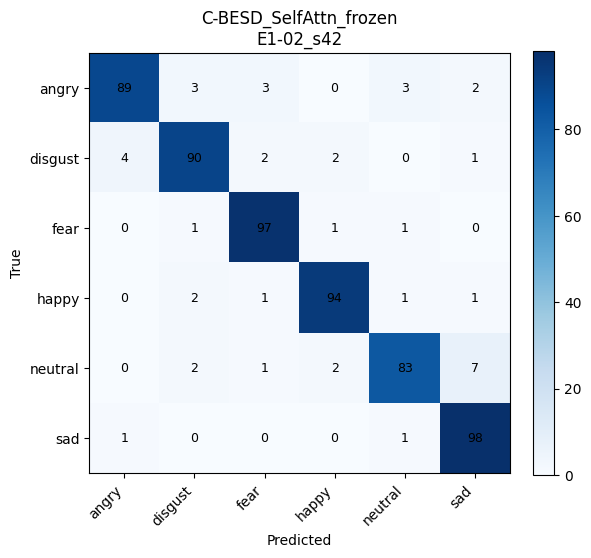
\includegraphics[width=0.45\textwidth]{../figures/cm_C-BESD_SelfAttn_frozen.png}
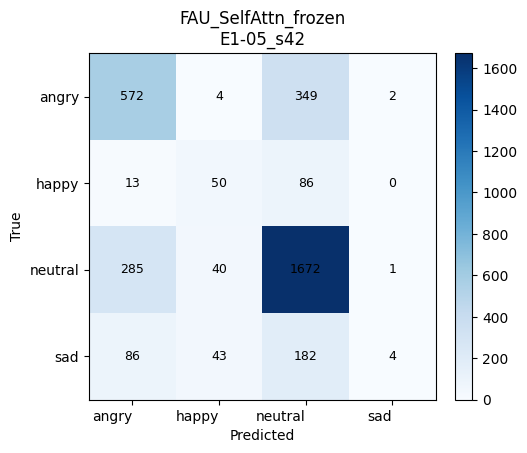
\includegraphics[width=0.45\textwidth]{../figures/cm_FAU_SelfAttn_frozen.png}
\caption{Confusion matrices for C-BESD (left) and FAU Aibo (right), frozen WavLM with self-attention pooling (E1-02 and E1-05).}
\label{fig:cms}
\end{figure}
